\documentclass[a4paper]{jpconf}
\usepackage{graphicx}

\begin{document}
\title{Data Aggregation System - a system for information retrieval on demand over relational and non-relational distributed data sources}
\author{G. Ball$^1$, V. Kuznetsov$^2$, D. Evans$^3$ and S. Metson$^4$}

\address{$^1$ Imperial College London, London, UK}
\address{$^2$ Cornell University, Ithaca, New York, USA}
\address{$^3$ Fermilab, Batavia, Illinois, USA}
\address{$^4$ Bristol University, Bristol, UK}

\ead{gordon.ball@cern.ch, vkuznet@gmail.com}

\begin{abstract}
We present the Data Aggregation System, a system for information retrieval and aggregation from heterogenous sources of relational and non-relational data for the Compact Muon Solenoid experiment on the CERN Large Hadron Collider. The experiment currently has a number of organically-developed data sources, including front-ends to a number of different relational databases and non-database data services which do not share common data structures or APIs {\it (Application Programming Interfaces)}, and cannot at this stage be readily converged. DAS provides a single interface for querying all these services, a caching layer to speed up access to expensive underlying calls and the ability to merge records from different data services pertaining to a single primary key.
\end{abstract}

\section{Introduction}

In 2010, data taking at the CMS experiment began in earnest, with approximately $42pb^{-1}$ of proton-proton collision data recorded at the time of writing. At full data-taking rates, this is expected to produce around 5PB of raw and reconstructed data per year. Associated with this is around 1TB per year of metadata, such as data locations, dataset descriptions and machine conditions.

Each of these metadata aspects are stored into a specialised system, using a variety of different technologies. Each provides specialised interfaces to query the specific metadata stored. In the pre-data-taking epoch, this situation was satisfactory as most systems were used in isolation and only then by experts. However, in the data-taking era users regularly need to perform queries across multiple data services (for example, to look up the recorded luminosity, machine conditions and software configuration for a particular dataset) which prove very expensive to serve under the existing model. DAS simplifies data look-up to end users by providing a single point of access and provides a caching layer to data services.

Although designed in the context of the CMS experiment, DAS itself does not make any experiment-specific assumptions about the data services it handles and is generalisable to other similar situations~\cite{drsg}.

\section{Architecture \& Implementation}

\begin{figure}
\begin{center}
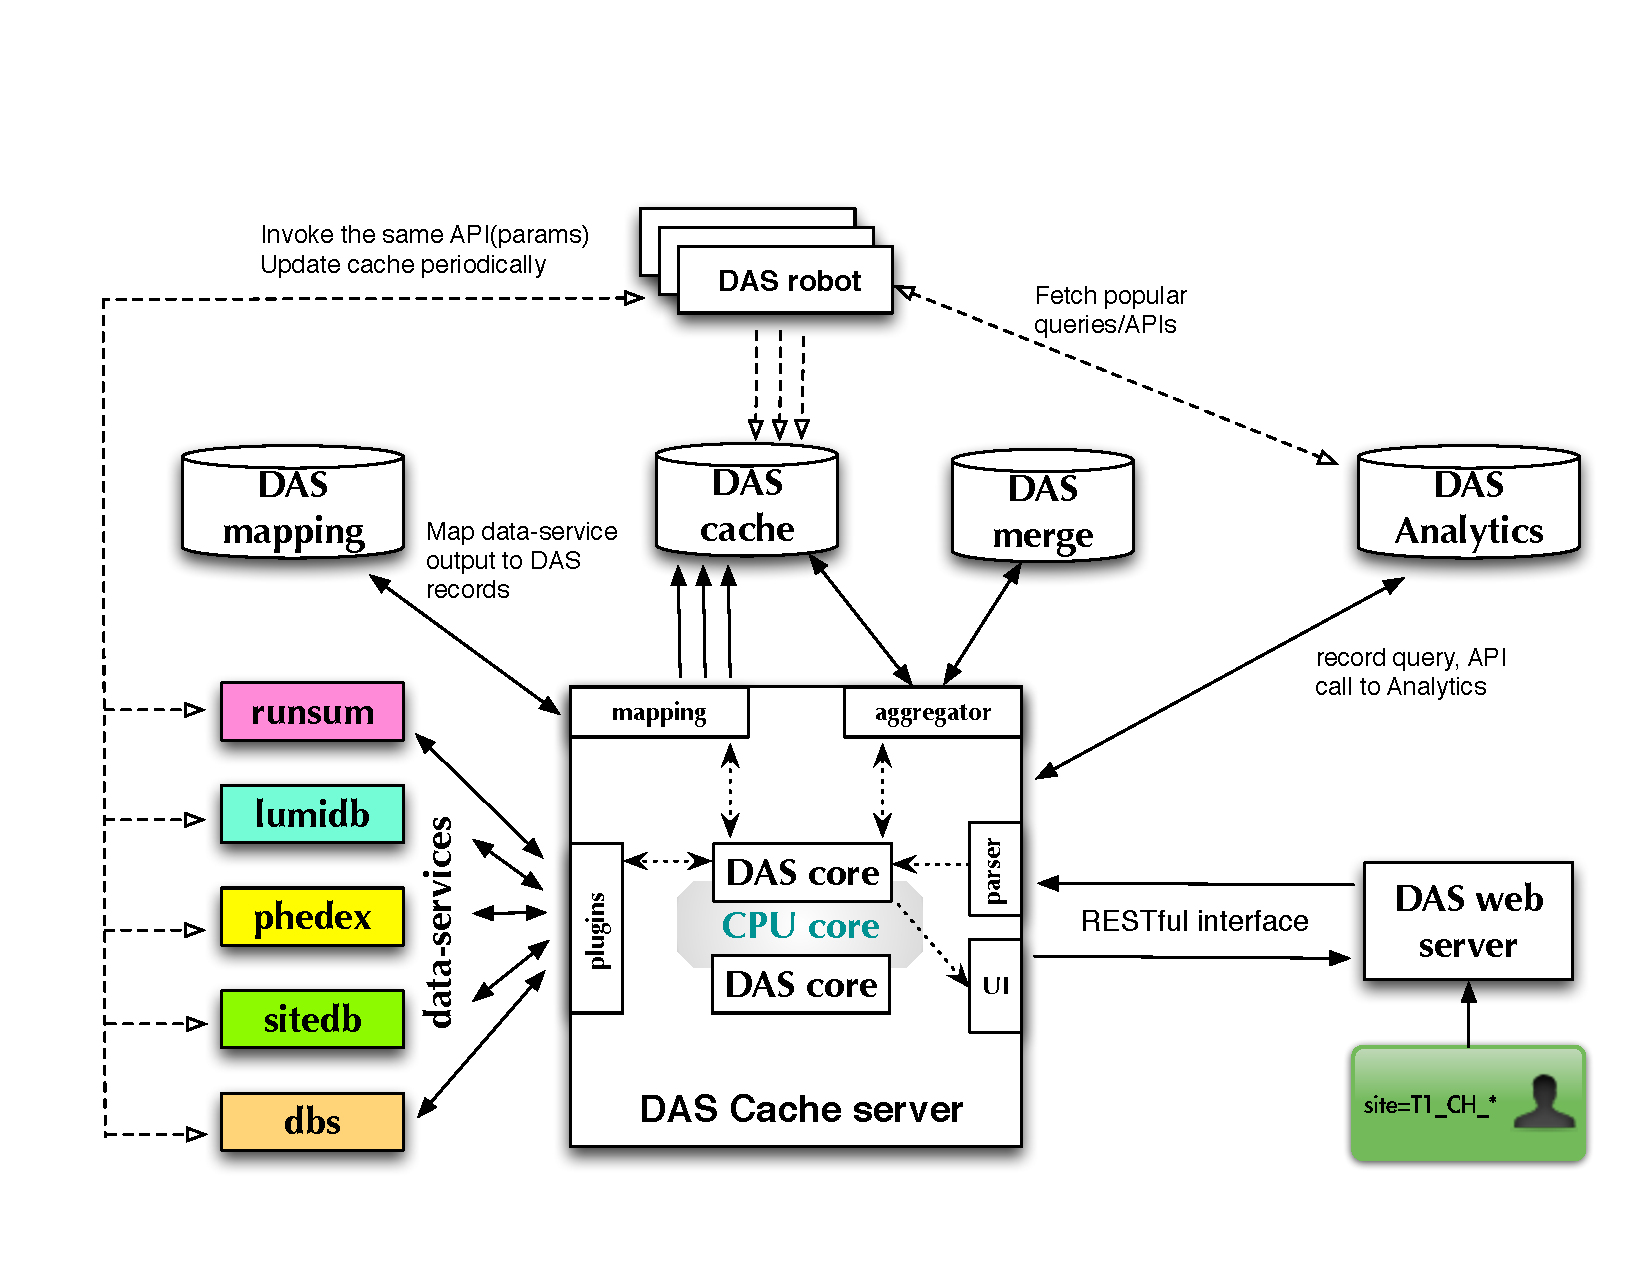
\includegraphics[width=0.6\textwidth]{DAS_Cache_and_Analytics}
\end{center}
\caption{\label{dasarch}DAS architecture, showing the relationships between \emph{web server}, \emph{cache server}, \emph{analytics}, \emph{data services} and MongoDB (\emph{cache} and \emph{merge}).}
\end{figure}

DAS is designed as an additional layer on top of a heterogenous ecosystem of existing CMS data services.
 
The architecture of DAS was designed as a series of independent components, which can scale from all running on a single node to multiple nodes and duplicate components, as necessary (Fig.~\ref{dasarch}). An initial description of the architecture, choice of technology and comparison with similar systems was given in \cite{das2010}. Here we present further development of the query language (Sec.~\ref{dasql}), analytics (Sec.~\ref{analytics}) and initial benchmark results (Sec.~\ref{benchmarks}).

The \emph{web server} handles user sessions, whether they originate from a browser or automated scripts. Queries made here are passed onto the \emph{cache server} for processing, during which time the \emph{web server} periodically polls for the current status and displays it to the user by AJAX {\it (Asynchronous Javascript and XML)}, until the request is completed. An MD5 hash of the input query is used to identify the correct output (and hence multiple users making identical queries will only result in a single worker thread doing the processing). Methods are provided here for output in machine-readable formats as well as human-readable formatting.

The \emph{cache server} consists of a pool of worker threads which handle the DAS queries received from the web front-end. Each query is handled entirely by a single thread. The worker thread first parses a text-based query from the DAS Query Language (Sec.~\ref{dasql}) into an internal representation. The query is then analysed to identify the set of data service APIs which are relevant. The \emph{cache} is checked for items of data matching the query, or data that would form a superset of the query. If any data cannot be found, the relevant service (Sec.~\ref{services}) is called to fetch and transform the data, and insert it into the raw cache (Sec.~\ref{cachemerge}). Once all the data is in the raw cache, records sharing common keys are merged together into a single document, which is stored in the merge cache. If any additional data processing has been specified in the query, it is performed on the merged document before being returned.

The \emph{cache} consists of one or more MongoDB~\cite{mongodb} shards. MongoDB is a document store which natively stores the JSON {\it (Javascript Object Notation)} documents DAS uses as its internal representation. This is used both for the primary record stores (the \emph{raw} and \emph{merged} caches) and for the ancillary databases required by DAS, such as storing the server logs, analytics data and mapping between keys. MongoDB also provides GridFS~\cite{gridfs}, which DAS uses to store otherwise oversize documents, typically the result of merging large numbers of raw documents together. The choice of a document store instead of a traditional relational database was driven by the need to be able to store and subsequently query individual members of the deeply-nested data structures that DAS handles, the structure of which are not known until run-time. We tested the CouchDB~\cite{couchdb} and MongoDB document stores for this purpose; we found the latter to have better performance in our use-case, better scalability across multiple nodes and a query model more compatible with our own.

The \emph{analytics server} provides a facility for scheduling regular tasks. The rest of DAS operates only when triggered by user input, and although some clean-up is performed at run-time (such as discarded expired records) it is also necessary to have a facility for running asynchronous operations. Analytics consists of a task scheduler and a pool of workers which execute the tasks. This is done independently of the \emph{cache server}, so heavy analytics tasks will not interfere with end-user use.

DAS assumes that the data in the cache can be recreated from the original data sources at any time, and thus it can function with a limited amount of space by deleting old data, nor does it require backup of this space. The design assumes the total number of records to be $O(5M)$, and MongoDB is capable of effectively functioning with collections of this size. Furthermore,  only a fraction would be expected to be resident in the cache at any one time.

DAS is designed as an entirely read-only system, with no ability to write data back to the underlying services, which simplifies the requirements for authentication and validation that this would otherwise require.

A random subset of results retrieved by DAS are examined to learn which data members are returned by which underlying queries, so that the web interface can suggest which input DAS keys will find the desired result.

The non-MongoDB parts of DAS are entirely written in python. Using python does come with a performance penalty but it allows for a fast development cycle, access to a number of useful libraries and is consistent with other CMS web projects.

\subsection{\label{dasql}DAS Query Language}

DAS queries are made in a custom text-based language. Work originally centred on an extended version of the query language already developed for the CMS Dataset Bookkeeping Service~\cite{dbsql} but the syntax was found unsuitable. The DAS syntax broadly resembles using pipes and commands in a UNIX shell, albeit with entirely dissimilar implementation.

Queries are parsed using the PLY~\cite{ply} parser for tokenising and lexical analysis, with a caching layer for previously parsed queries. The query is internally represented as a python dictionary containing the conditions and any additional operations.

A query is structured:

\begin{verbatim}
conditions | filters | aggregators OR map-reduce 
\end{verbatim}

To make a query, a user must know which \emph{DAS key} describes the data they are seeking. DAS keys describe a single logical object, descriptions of which may exist in multiple data services. Examples of DAS keys used for CMS include \textbf{dataset}, \textbf{run\_number} and \textbf{person}. In most cases these are the same names used by the data services, but DAS hides small differences in data service terminologies (eg, \textbf{run\_number} is variously called \textbf{runNumber} and \textbf{Run} by different services).

The \emph{conditions} consist of one or more DAS keys, optionally followed by an operator and operand. Examples of queries include:

\begin{verbatim}
city=Geneva
dataset site=institute.ac.uk
run in [123, 456]
\end{verbatim}

The conditions determine the total data for the query, but since this may still be a significant volume of data (or contain a significant number of fields of no interest to the user), further operations can be performed on the data.

\emph{Filters} are commands that either eliminate complete data records or prune data members within a record. At this time only two are provided; \emph{grep} works similarly to the UNIX command of the same name, filtering all but the given data members from the output, and \emph{unique} eliminates duplicate records. This is implemented by converting the filter conditions into MongoDB query format.

\emph{Aggregators} are functions which run over all the selected (and filtered, if applicable) records, summarising their contents. The basic aggregators available are simple numerical functions like \emph{sum}, \emph{count} and \emph{avg}, which perform the named aggregation over all data members of a given name. Aggregation is implemented using python coroutines.

An example of a ``complete'' query might be:

\begin{verbatim}
block dataset=/a/b/c* | grep block.size | sum(block.size), max(block.size)
\end{verbatim}

The set of available filters and aggregators is likely to grow in accordance with user needs. For more complex use-cases, it is possible to run a javascript map-reduce function on the MongoDB cache server. DAS QL does not allow functions to be specified, so such functions are written in advance and stored in the cache, and their execution requested with an alias.

\subsection{\label{services}Services}

Almost any source of information can be incorporated in DAS, such as an SQL database cursor, a command called in a subshell or an HTML page scraper, but in practice most data services used by DAS are APIs accessed over HTTP and returning data in JSON or XML format.

Each data service is described in a mapping document (supplied in YAML~\cite{yaml} format) which describes the functions available, the mapping from input DAS keys to actual arguments, and finally a mapping from the returned keys back to DAS keys. For a service accessed over HTTP and using a standard format, adding a new service only requires this mapping.

For more complex cases, such as those for which authentication is required, or for different source types a plugin must be written which translates DAS requests into the necessary calls, and then transforms the output into DAS JSON documents.

The mapping document may also specify presentation information which is used to produce more human-friendly output by mapping key names to descriptions.

When a query for which no exact match exists in the cache is received, the set of input DAS keys is considered to determine which services and their respective APIs to invoke. If the query consists only of keys with associated conditions, the relevant APIs are all those for which the accepted DAS keys are either equal or a superset of the input keys. If no API matches the set of input queries, it is decomposed into multiple sub-queries.

Before an API query is made, a check is made for existence of a superset query already in the cache, if wildcarding is supported by the service.

\subsection{\label{cachemerge}Caching \& Merging}

Data in DAS is principally stored in two seperate collections; the raw and merged caches.

Two types of data are stored in the raw cache; the documents returned by the respective APIs and documents describing the current status of queries. The latter serves as the central record for a query, holding the original query, description of the APIs called, status of the processing and a common key with all the results documents.

Once all the data for a query is available in the raw cache, a merged record is created for each primary DAS key. Merged documents may exceed the maximum size possible for MongoDB records, in which case they are stored using GridFS and a reference to them stored in the merged cache instead.

\subsection{\label{analytics}Analytics}

The DAS analytics system is a daemon that schedules and executes small tasks that access the DAS document store. This can be used to perform prosaic maintainance tasks, such as cleaning out expired data or pruning still-valid data if space becomes limited, but the main function is to analyse the queries received by DAS to provide information to developers and to perform automated cache optimisation.

The caching aspect of DAS is meant to reduce the latency users experience when performing complex, cross-service queries, but since the data in question usually has TTL of less than an hour users will relatively often find that the data they request is not in the cache and must be fetched on demand.

The analytics system hence tries to identify the most popular user queries and ensure that they are always resident in the cache and thus available for real-time retrieval, whatever the actual fetch latency may have been.

It is vital to the success of DAS, both in terms of user experience and system load, that the majority of all queries can be served from the cache. To ensure this, we must have a good pre-fetching strategy that maintains itself based on the actions of users.

Tasks that run on the analytics system may be divided into query analysis and cache populators. The former run infrequently, performing expensive (both in terms of processing and MongoDB access) analysis operations. Having identified the set of queries they wish to maintain, they spawn simpler populator tasks that schedule themselves to pre-empt each expiry of the specified data and perform an update, until the next time the analyser runs and the priorities may be altered.

A simple example of an analyser is designated \emph{ValueHotspot}, and is designed to run every few hours, identifying popular arguments to a given DAS key. Upon each invocation, the set of queries issued since the last invocation which reference the specified key is identified, and a count of each argument made. This is then combined with summary documents from previous invocations (containing the same information for those epochs) to calculate a 30-day moving average. The top $15\%$ most-used arguments are selected, which based on past results represent about $50\%$ of all queries are then kept in the cache until the analyser next runs.

There are a large number of possible future analysis strategies (such as the time structure throughout a week of certain types of queries, automatically pre-fetching information about new datasets as they are released or considering a metric based on total preventible latency rather than total numbers of calls), but some experience with actual users is needed to determine what will actually prove useful.

\section{\label{benchmarks}Benchmarks}

\begin{figure}
\begin{center}
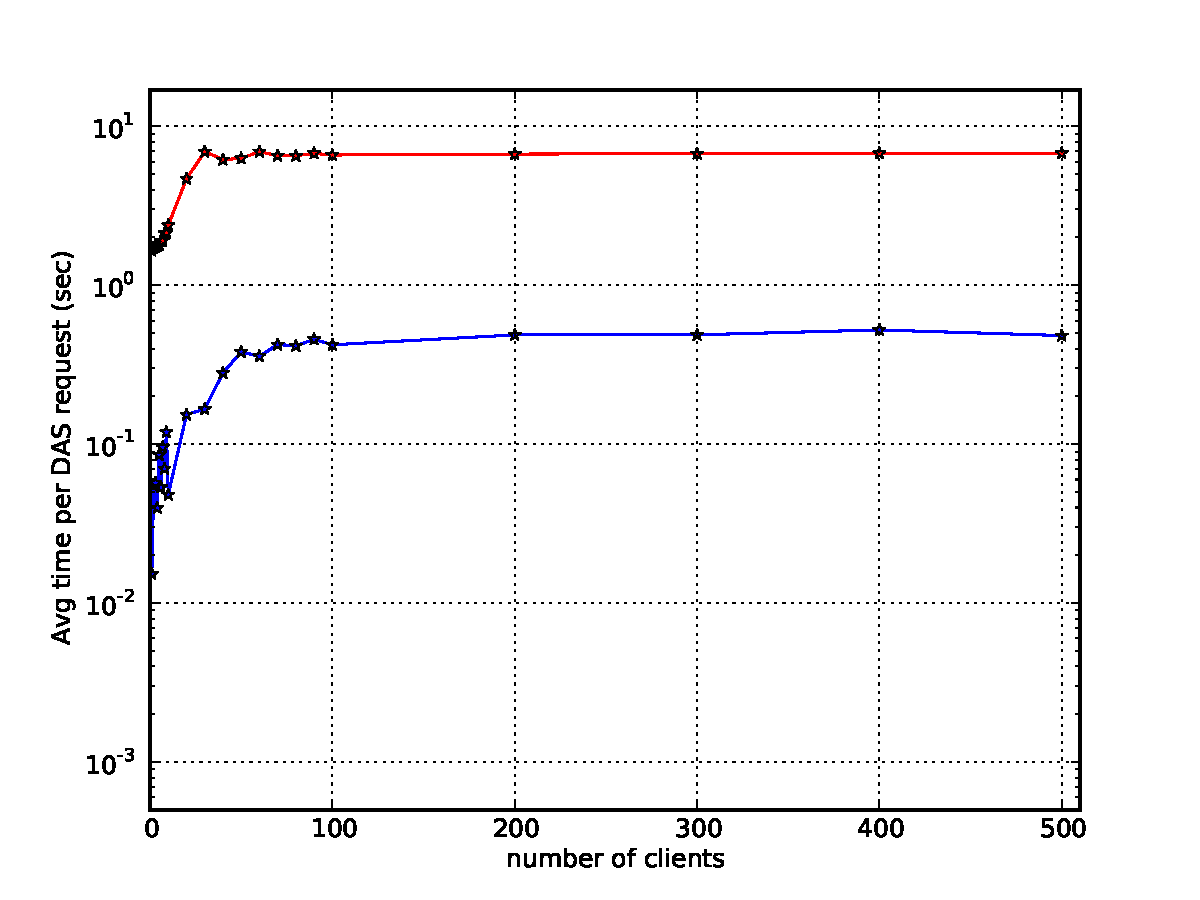
\includegraphics[width=0.6\textwidth]{das_vs_mongo_fully_random}
\end{center}
\caption{\label{dasbench}Benchmark showing the average latency for fetching a single randomly-selected document from a wildcard query, with a given number of parallel clients. The cache contains $5\times10^7$ records. The red triangles show the performance of the complete DAS stack, and the blue stars the time spent by MongoDB.}
\end{figure}

To benchmark DAS performance, we used a 64-bit linux node with 8 cores (each 2.33GhZ) and 16GB of RAM, which we would expect to be typical of the hardware DAS would use in production. All DAS systems and MongoDB share this node.

%Testing was performed with the cache pre-populated with approximately $5\times10^7$ records (100 times the expected volume), consisting of \emph{block} records from the CMS PhEDEx~\cite{phedex} and DBS systems. We test with up to 500 clients making requests in parallel. Each client requests one random record from the entire result set (which will test the time required for DAS to process the query but largely exclude the time required to serialise a large output set), using queries of the form \verb block=/[a-z]* (past experience with the DBS system shows wildcard queries are very common, even when the user knows the complete string in question). Fig.~\ref{dasbench} shows the benchmark results.
Testing was performed with the cache pre-populated with approximately 
$5\times10^7$ records (100 times the expected volume), consisting 
of \emph{block} records from the CMS PhEDEx~\cite{phedex} and DBS 
systems. Each \emph{block} record is a JSON document with common keys, such as
\emph{name, nevents, nfiles, replica}, etc.
We test with up to 500 clients making requests in parallel. 
Each client requests a random wildcard query, e.g. \verb block=/a* , and fetches one random
record from the returned set (which will test the time required for DAS to parse the 
query and access the cache but largely exclude the time required to serialise a large 
output set). No additional operations were done during this step.
Fig.~\ref{dasbench} shows the benchmark results.

\section{Future Work}

We are currently in process of deploying DAS in the production environment for beta testing. The main development focus at this time is to increase the scope of possible queries, both by adding additional services and increasing the number of APIs supported for existing services. Support currently exists to some degree for the CMS services DBS, PhEDEx, SiteDB, Tier-0, LumiDB, RunRegistry, Dashboard and Overview. Most of these however only have a few APIs described by the DAS mapping, and to ensure usefulness to users we need to support as many of the queries supported by their original interfaces as possible.

\ack

This work was supported by the National Science Foundation, contract No. PHY-0757894, and the Department of Energy of the United States of America.

This work was supported by the Science and Technology Facilities Council, UK.

\appendix

\section*{References}
\begin{thebibliography}{9}
\bibitem{drsg} DISCOVER RSG {\it http://drsg.cac.cornell.edu/content/drsg-pilot-projects}
\bibitem{das2010} Kuznetsov V, Evans D and Metson S 2010 The CMS data aggregation system {\it Procedia Comp. Sci.} {\bf 1} 1529-37
\bibitem{mongodb} MongoDB, a scalable, high-performance, open-source, document-orientated database {\it http://www.mongodb.org/}
\bibitem{gridfs} MongoDB GridFS {\it http://www.mongodb.org/display/DOCS/GridFS}
\bibitem{couchdb} Apache CouchDB {\it http://couchdb.apache.org/}
\bibitem{dbsql} Kuznetsov V, Riley D, Afaq A, Sekhri V, Guo Y and Lueking L 2009 The CMS DBS query language {\it CHEP}
\bibitem{ply} Python Lex-Yacc {\it http://www.dabeaz.com/ply/}
\bibitem{yaml} YAML ain't markup language {\it http://www.yaml.org/}
\bibitem{phedex} Rehn J, Barrass T, Bonacorsi D, Hernandez J, Semeniouk I, Tuura L and Wu Y 2006 PhEDEx high-throughput data transfer management system {\it CHEP}
\end{thebibliography}
\end{document}
